


\tikzset{every picture/.style={line width=0.75pt}} %set default line width to 0.75pt        

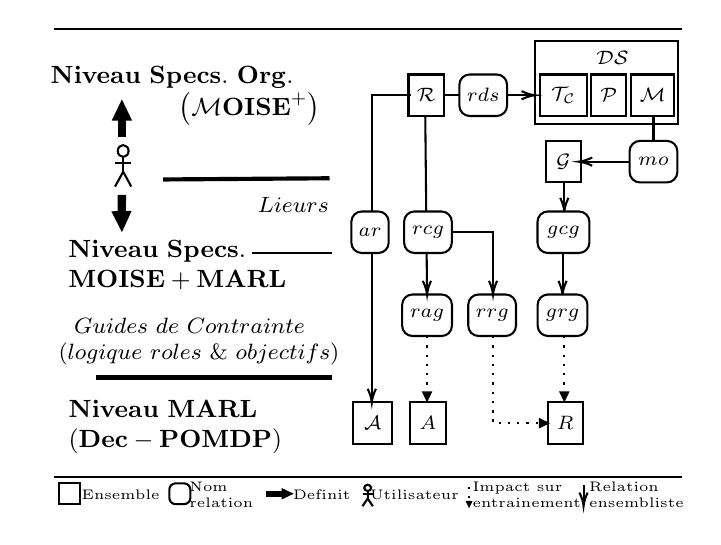
\begin{tikzpicture}[x=0.75pt,y=0.75pt,yscale=-1,xscale=1]
%uncomment if require: \path (0,4572); %set diagram left start at 0, and has height of 4572

%Straight Lines [id:da49405221005902566] 
\draw [line width=1.5]    (230.7,4255.58) -- (310.89,4255) ;
%Straight Lines [id:da9343410580129854] 
\draw    (466.97,4225) -- (466.97,4247) -- (432.9,4247) ;
\draw [shift={(430.9,4247)}, rotate = 360] [color={rgb, 255:red, 0; green, 0; blue, 0 }  ][line width=0.75]    (6.56,-1.97) .. controls (4.17,-0.84) and (1.99,-0.18) .. (0,0) .. controls (1.99,0.18) and (4.17,0.84) .. (6.56,1.97)   ;
%Straight Lines [id:da7846025645580084] 
\draw [line width=1.5]    (198.28,4351) -- (312.31,4351) ;
%Straight Lines [id:da47840194291314075] 
\draw    (273.57,4290.8) -- (312.31,4290.8) ; % ttt
%Straight Lines [id:da6114502168118399] 
\draw    (178,4399) -- (480.95,4399) ;
%Straight Lines [id:da560434509782435] 
\draw    (178,4183) -- (480.81,4183) ;
%Straight Lines [id:da20789839643202224] 
\draw    (350.16,4215) -- (331.27,4215) -- (331.27,4361) ;
\draw [shift={(331.27,4363)}, rotate = 270] [color={rgb, 255:red, 0; green, 0; blue, 0 }  ][line width=0.75]    (6.56,-1.97) .. controls (4.17,-0.84) and (1.99,-0.18) .. (0,0) .. controls (1.99,0.18) and (4.17,0.84) .. (6.56,1.97)   ;
%Straight Lines [id:da39528654489791415] 
\draw    (357.03,4281) -- (389.67,4281) -- (389.67,4309) ;
\draw [shift={(389.67,4311)}, rotate = 270] [color={rgb, 255:red, 0; green, 0; blue, 0 }  ][line width=0.75]    (6.56,-1.97) .. controls (4.17,-0.84) and (1.99,-0.18) .. (0,0) .. controls (1.99,0.18) and (4.17,0.84) .. (6.56,1.97)   ;
%Straight Lines [id:da03646449435518195] 
\draw [line width=0.75]  [dash pattern={on 0.84pt off 2.51pt}]  (357.89,4331) -- (357.89,4360) ;
\draw [shift={(357.89,4363)}, rotate = 270] [fill={rgb, 255:red, 0; green, 0; blue, 0 }  ][line width=0.08]  [draw opacity=0] (5.36,-2.57) -- (0,0) -- (5.36,2.57) -- cycle    ;
%Straight Lines [id:da12277835004093052] 
\draw    (424.03,4257) -- (424.03,4269) ;
\draw [shift={(424.03,4271)}, rotate = 270] [color={rgb, 255:red, 0; green, 0; blue, 0 }  ][line width=0.75]    (6.56,-1.97) .. controls (4.17,-0.84) and (1.99,-0.18) .. (0,0) .. controls (1.99,0.18) and (4.17,0.84) .. (6.56,1.97)   ;
%Straight Lines [id:da31168572322613364] 
\draw [line width=0.75]  [dash pattern={on 0.84pt off 2.51pt}]  (424.03,4331) -- (424.03,4360) ;
\draw [shift={(424.03,4363)}, rotate = 270] [fill={rgb, 255:red, 0; green, 0; blue, 0 }  ][line width=0.08]  [draw opacity=0] (5.36,-2.57) -- (0,0) -- (5.36,2.57) -- cycle    ;
%Straight Lines [id:da922872392878513] 
\draw [line width=0.75]  [dash pattern={on 0.84pt off 2.51pt}]  (389.67,4331) -- (389.67,4373) -- (414.15,4373) ;
\draw [shift={(417.15,4373)}, rotate = 180] [fill={rgb, 255:red, 0; green, 0; blue, 0 }  ][line width=0.08]  [draw opacity=0] (5.36,-2.57) -- (0,0) -- (5.36,2.57) -- cycle    ;
%Straight Lines [id:da7338110321736906] 
\draw [line width=0.75]  [dash pattern={on 0.84pt off 2.51pt}]  (378.15,4403.7) -- (378.15,4411) ;
\draw [shift={(378.15,4414)}, rotate = 270] [fill={rgb, 255:red, 0; green, 0; blue, 0 }  ][line width=0.08]  [draw opacity=0] (3.57,-1.72) -- (0,0) -- (3.57,1.72) -- cycle    ;
%Straight Lines [id:da2555753099570559] 
\draw    (433.29,4402.98) -- (433.29,4411) ;
\draw [shift={(433.29,4413)}, rotate = 270] [color={rgb, 255:red, 0; green, 0; blue, 0 }  ][line width=0.75]    (6.56,-1.97) .. controls (4.17,-0.84) and (1.99,-0.18) .. (0,0) .. controls (1.99,0.18) and (4.17,0.84) .. (6.56,1.97)   ;
%Shape: Ellipse [id:dp4933051166226825] 
\draw   (208.86,4241.86) .. controls (208.86,4240.28) and (210.03,4239) .. (211.48,4239) .. controls (212.92,4239) and (214.09,4240.28) .. (214.09,4241.86) .. controls (214.09,4243.44) and (212.92,4244.71) .. (211.48,4244.71) .. controls (210.03,4244.71) and (208.86,4243.44) .. (208.86,4241.86) -- cycle ;
%Straight Lines [id:da0026830528705521495] 
\draw    (211.48,4244.71) -- (211.48,4251.86) ;
%Straight Lines [id:da4879750022905194] 
\draw    (211.48,4251.86) -- (207.56,4259) ;
%Straight Lines [id:da13833288810166278] 
\draw    (211.48,4251.86) -- (215.39,4259) ;
%Straight Lines [id:da8484131725046102] 
\draw    (215.39,4247.57) -- (207.56,4247.57) ;

%Straight Lines [id:da3014432179926261] 
\draw [line width=2.25]    (280.41,4407) -- (288.6,4407) ;
\draw [shift={(293.6,4407)}, rotate = 180] [fill={rgb, 255:red, 0; green, 0; blue, 0 }  ][line width=0.08]  [draw opacity=0] (5.72,-2.75) -- (0,0) -- (5.72,2.75) -- cycle    ;
%Shape: Ellipse [id:dp19398062215243272] 
\draw   (327.62,4404.17) .. controls (327.62,4403.36) and (328.36,4402.7) .. (329.28,4402.7) .. controls (330.2,4402.7) and (330.95,4403.36) .. (330.95,4404.17) .. controls (330.95,4404.99) and (330.2,4405.65) .. (329.28,4405.65) .. controls (328.36,4405.65) and (327.62,4404.99) .. (327.62,4404.17) -- cycle ;
%Straight Lines [id:da13358439414356815] 
\draw    (329.28,4405.65) -- (329.28,4409.32) ;
%Straight Lines [id:da02722538513278816] 
\draw    (329.28,4409.32) -- (326.79,4413) ;
%Straight Lines [id:da7818198115272541] 
\draw    (329.28,4409.32) -- (331.78,4413) ;
%Straight Lines [id:da2988198411812537] 
\draw    (331.78,4407.12) -- (326.79,4407.12) ;

%Straight Lines [id:da28727926162240225] 
\draw    (357.03,4225) -- (357.87,4309) ;
\draw [shift={(357.89,4311)}, rotate = 269.43] [color={rgb, 255:red, 0; green, 0; blue, 0 }  ][line width=0.75]    (6.56,-1.97) .. controls (4.17,-0.84) and (1.99,-0.18) .. (0,0) .. controls (1.99,0.18) and (4.17,0.84) .. (6.56,1.97)   ;
%Straight Lines [id:da7563430741621355] 
\draw    (423.17,4291) -- (423.17,4309) ;
\draw [shift={(423.17,4311)}, rotate = 270] [color={rgb, 255:red, 0; green, 0; blue, 0 }  ][line width=0.75]    (6.56,-1.97) .. controls (4.17,-0.84) and (1.99,-0.18) .. (0,0) .. controls (1.99,0.18) and (4.17,0.84) .. (6.56,1.97)   ;
%Shape: Rectangle [id:dp032787025179332296] 
\draw   (233.72,4405) .. controls (233.72,4403.34) and (235.07,4402) .. (236.72,4402) -- (240.85,4402) .. controls (242.5,4402) and (243.85,4403.34) .. (243.85,4405) -- (243.85,4409) .. controls (243.85,4410.66) and (242.5,4412) .. (240.85,4412) -- (236.72,4412) .. controls (235.07,4412) and (233.72,4410.66) .. (233.72,4409) -- cycle ;
%Straight Lines [id:da6562984445922673] 
\draw    (365.62,4215) -- (407.97,4215) ;
\draw [shift={(409.97,4215)}, rotate = 180] [color={rgb, 255:red, 0; green, 0; blue, 0 }  ][line width=0.75]    (6.56,-1.97) .. controls (4.17,-0.84) and (1.99,-0.18) .. (0,0) .. controls (1.99,0.18) and (4.17,0.84) .. (6.56,1.97)   ;
%Shape: Rectangle [id:dp7533146593468494] 
\draw   (409.97,4189) -- (478.99,4189) -- (478.99,4229) -- (409.97,4229) -- cycle ;
%Straight Lines [id:da6163625666300567] 
\draw [line width=3]    (210.87,4235) -- (210.87,4223) ;
\draw [shift={(210.87,4217)}, rotate = 90] [fill={rgb, 255:red, 0; green, 0; blue, 0 }  ][line width=0.08]  [draw opacity=0] (10.18,-4.89) -- (0,0) -- (10.18,4.89) -- cycle    ;
%Straight Lines [id:da7349066590871605] 
\draw [line width=3]    (210.87,4263) -- (210.77,4275.37) ;
\draw [shift={(210.87,4281)}, rotate = 268.92] [fill={rgb, 255:red, 0; green, 0; blue, 0 }  ][line width=0.08]  [draw opacity=0] (10.18,-4.89) -- (0,0) -- (10.18,4.89) -- cycle    ;
%Shape: Rectangle [id:dp5258359496766027] 
\draw   (180.78,4402) -- (190.9,4402) -- (190.9,4412) -- (180.78,4412) -- cycle ;


% Text Node
\draw  [fill={rgb, 255:red, 255; green, 255; blue, 255 }  ,fill opacity=1 ]  (346.82,4276) .. controls (346.82,4273.24) and (349.06,4271) .. (351.82,4271) -- (364.82,4271) .. controls (367.58,4271) and (369.82,4273.24) .. (369.82,4276) -- (369.82,4286) .. controls (369.82,4288.76) and (367.58,4291) .. (364.82,4291) -- (351.82,4291) .. controls (349.06,4291) and (346.82,4288.76) .. (346.82,4286) -- cycle  ;
\draw (358.32,4281) node  [font=\scriptsize] [align=left] {$\displaystyle \boldsymbol{rcg}$};
% Text Node
\draw    (436.89,4205) -- (453.89,4205) -- (453.89,4225) -- (436.89,4225) -- cycle  ;
\draw (445.39,4215) node  [font=\scriptsize] [align=left] {$\displaystyle \mathcal{P}$};
% Text Node
\draw    (412.16,4205) -- (435.16,4205) -- (435.16,4225) -- (412.16,4225) -- cycle  ;
\draw (423.66,4215) node  [font=\scriptsize] [align=left] {$\displaystyle \mathcal{T_{C}}$};
% Text Node
\draw    (456.04,4205) -- (477.04,4205) -- (477.04,4225) -- (456.04,4225) -- cycle  ;
\draw (466.54,4215) node  [font=\scriptsize] [align=left] {$\displaystyle \mathcal{M}$};
% Text Node
\draw (447.21,4197) node  [font=\scriptsize] [align=left] {$\displaystyle \mathcal{DS}$};
% Text Node
\draw  [fill={rgb, 255:red, 255; green, 255; blue, 255 }  ,fill opacity=1 ]  (373.44,4210) .. controls (373.44,4207.24) and (375.68,4205) .. (378.44,4205) -- (391.44,4205) .. controls (394.2,4205) and (396.44,4207.24) .. (396.44,4210) -- (396.44,4220) .. controls (396.44,4222.76) and (394.2,4225) .. (391.44,4225) -- (378.44,4225) .. controls (375.68,4225) and (373.44,4222.76) .. (373.44,4220) -- cycle  ;
\draw (384.94,4215) node  [font=\scriptsize] [align=left] {$\displaystyle \boldsymbol{rds}$};
% Text Node
\draw (258.78,4407.5) node  [font=\tiny] [align=left] {Nom\\relation};
% Text Node
\draw (210.23,4407.5) node  [font=\tiny] [align=left] {Ensemble};
% Text Node
\draw (351.82,4407.5) node  [font=\tiny] [align=left] {Utilisateur};
% Text Node
\draw (307.16,4407.5) node  [font=\tiny] [align=left] {Definit};
% Text Node
\draw (458.79,4407.5) node  [font=\tiny] [align=left] {Relation\\ensembliste};
% Text Node
\draw (405.9,4407.5) node  [font=\tiny] [align=left] {Impact sur\\entrainement};
% Text Node
\draw    (349.82,4363) -- (366.82,4363) -- (366.82,4383) -- (349.82,4383) -- cycle  ;
\draw (358.32,4373) node  [font=\scriptsize] [align=left] {$\displaystyle \boldsymbol{A}$};
% Text Node
\draw    (415.95,4363) -- (432.95,4363) -- (432.95,4383) -- (415.95,4383) -- cycle  ;
\draw (424.45,4373) node  [font=\scriptsize] [align=left] {$\displaystyle \boldsymbol{R}$};
% Text Node
\draw    (322.2,4363) -- (341.2,4363) -- (341.2,4383) -- (322.2,4383) -- cycle  ;
\draw (331.7,4373) node  [font=\scriptsize] [align=left] {$\displaystyle \mathcal{A}$};
% Text Node
\draw  [fill={rgb, 255:red, 255; green, 255; blue, 255 }  ,fill opacity=1 ]  (411.17,4316) .. controls (411.17,4313.24) and (413.41,4311) .. (416.17,4311) -- (430.17,4311) .. controls (432.93,4311) and (435.17,4313.24) .. (435.17,4316) -- (435.17,4326) .. controls (435.17,4328.76) and (432.93,4331) .. (430.17,4331) -- (416.17,4331) .. controls (413.41,4331) and (411.17,4328.76) .. (411.17,4326) -- cycle  ;
\draw (423.17,4321) node  [font=\scriptsize] [align=left] {$\displaystyle \boldsymbol{grg}$};
% Text Node
\draw    (377.74,4316) .. controls (377.74,4313.24) and (379.98,4311) .. (382.74,4311) -- (395.74,4311) .. controls (398.5,4311) and (400.74,4313.24) .. (400.74,4316) -- (400.74,4326) .. controls (400.74,4328.76) and (398.5,4331) .. (395.74,4331) -- (382.74,4331) .. controls (379.98,4331) and (377.74,4328.76) .. (377.74,4326) -- cycle  ;
\draw (389.24,4321) node  [font=\scriptsize] [align=left] {$\displaystyle \boldsymbol{rrg}$};
% Text Node
\draw    (345.89,4316) .. controls (345.89,4313.24) and (348.13,4311) .. (350.89,4311) -- (364.89,4311) .. controls (367.65,4311) and (369.89,4313.24) .. (369.89,4316) -- (369.89,4326) .. controls (369.89,4328.76) and (367.65,4331) .. (364.89,4331) -- (350.89,4331) .. controls (348.13,4331) and (345.89,4328.76) .. (345.89,4326) -- cycle  ;
\draw (357.89,4321) node  [font=\scriptsize] [align=left] {$\displaystyle \boldsymbol{rag}$};
% Text Node
\draw (247.98,4333.5) node  [font=\footnotesize] [align=left] {$\displaystyle  \begin{array}{{>{\displaystyle}l}}
\ \ \boldsymbol{Guides\ de\ Contrainte}\\
( logique\ roles\ \&\ objectifs)
\end{array}$};
% Text Node
\draw  [fill={rgb, 255:red, 255; green, 255; blue, 255 }  ,fill opacity=1 ]  (411.1,4276) .. controls (411.1,4273.24) and (413.33,4271) .. (416.1,4271) -- (431.1,4271) .. controls (433.86,4271) and (436.1,4273.24) .. (436.1,4276) -- (436.1,4286) .. controls (436.1,4288.76) and (433.86,4291) .. (431.1,4291) -- (416.1,4291) .. controls (413.33,4291) and (411.1,4288.76) .. (411.1,4286) -- cycle  ;
\draw (423.6,4281) node  [font=\scriptsize] [align=left] {$\displaystyle \boldsymbol{gcg}$};
% Text Node
\draw  [fill={rgb, 255:red, 255; green, 255; blue, 255 }  ,fill opacity=1 ]  (321.41,4276) .. controls (321.41,4273.24) and (323.65,4271) .. (326.41,4271) -- (334.41,4271) .. controls (337.17,4271) and (339.41,4273.24) .. (339.41,4276) -- (339.41,4286) .. controls (339.41,4288.76) and (337.17,4291) .. (334.41,4291) -- (326.41,4291) .. controls (323.65,4291) and (321.41,4288.76) .. (321.41,4286) -- cycle  ;
\draw (330.41,4281) node  [font=\scriptsize] [align=left] {$\displaystyle \boldsymbol{ar}$};
% Text Node
\draw  [fill={rgb, 255:red, 255; green, 255; blue, 255 }  ,fill opacity=1 ]  (455.47,4242) .. controls (455.47,4239.24) and (457.71,4237) .. (460.47,4237) -- (473.47,4237) .. controls (476.23,4237) and (478.47,4239.24) .. (478.47,4242) -- (478.47,4252) .. controls (478.47,4254.76) and (476.23,4257) .. (473.47,4257) -- (460.47,4257) .. controls (457.71,4257) and (455.47,4254.76) .. (455.47,4252) -- cycle  ;
\draw (466.97,4247) node  [font=\scriptsize] [align=left] {$\displaystyle \boldsymbol{mo}$};
% Text Node
\draw (237.59,4297.5) node  [font=\small] [align=left] {$\displaystyle  \begin{array}{{>{\displaystyle}l}}
\mathbf{Niveau\ Specs.}\\
\mathbf{MOISE+MARL}
\end{array}$};
% Text Node
\draw (236.64,4374.5) node  [font=\small] [align=left] {$\displaystyle  \begin{array}{{>{\displaystyle}l}}
\mathbf{Niveau\ MARL}\\
\mathbf{( Dec-POMDP)}
\end{array}$};
% Text Node
\draw    (348.96,4205) -- (365.96,4205) -- (365.96,4225) -- (348.96,4225) -- cycle  ;
\draw (357.46,4215) node  [font=\scriptsize] [align=left] {$\displaystyle \mathcal{R}$};
% Text Node
\draw (293.45,4268) node  [font=\footnotesize] [align=left] {$\displaystyle \boldsymbol{Lieurs}$};
% Text Node
\draw    (415.1,4237) -- (432.1,4237) -- (432.1,4257) -- (415.1,4257) -- cycle  ;
\draw (423.6,4247) node  [font=\scriptsize] [align=left] {$\displaystyle \mathcal{G}$};
% Text Node
\draw (241.59,4214.5) node  [font=\small] [align=left] {$\displaystyle  \begin{array}{{>{\displaystyle}l}}
\mathbf{{\displaystyle Niveau\ Specs.\ Org.}}\\
{\displaystyle \ \ \ \ \ \ \ \ \ \ \ \ \ \ \ \mathbf{\left(\mathcal{M}OISE^{+}\right)}}
\end{array}$};


\end{tikzpicture}